\section{Textsatz}
\subsection{Klassen und Bibliotheken}

\begin{frame}[fragile,t]
\frametitle{Dokumentklassen}
Jedes Dokument beginnt mit der Definition der Dokumentenklasse:
\begin{center}
\lstinline[style=Latex]+\documentclass[<Optionen>]{<Klasse>}+
\end{center}
\pause
Hier eine Liste verschiedener vordefinierter Klassen:\pause
\begin{itemize}[<+->]
  \item article
  \item report
%  \item letter
  \item book
  \item beamer
  \item amsbook, amsart % American Mathematical Society
  \item scrartcl, scrbook, scrreprt % Koma-Klassen
\end{itemize}
\end{frame}


\begin{frame}[fragile,t]
\frametitle{Dokumentklassen, Optionen}
Jedes Dokument beginnt mit der Definition der Dokumentenklasse:
\begin{center}
\lstinline[style=Latex]+\documentclass[<Optionen>]{<Klasse>}+
\end{center}
Hier eine Liste verschiedener Optionen:\pause
\begin{itemize}[<+->]
  \item 10pt, 11pt, 12pt: Schriftgröße
  \item a4paper, a5paper, letterpaper, \ldots: Papierformat
%  \item landscape: Querformat
%  \item onecolumn, twocolumn: Teilt das Papier in Spalten
%  \item oneside, twoside: Einseitiges / Zweiseitiges Papier
%  \item openright, openany: Wo dürfen Kapitel anfangen?
%  \item titlepage, notitlepage: ob eine seperate Titelseite eingefügt werden soll
%  \item draft, final: Bilder nur als Boxen
\end{itemize}
\end{frame}

\begin{frame}[fragile,t]
\frametitle{Beispiel: Erstellen einer Titelseite}
{\scriptsize
\begin{lstlisting}[style=latex]
\begin{document}

\begin{titlepage}
\begin{center}
~\\[2cm]
\huge{\textbf{[Thema]\\[4cm]}}
\Large{Bachelorarbeit zur Erlangung des Grades\\
Bachelor of Science (B.Sc.)\\
im Studiengang Volkswirtschaftslehre\\
an der Rheinischen Friedrich-Wilhelms-Universität Bonn\\[7cm]
Themensteller/in: [Name des/r Betreuers/in]
\vfill
% Ende der Seite
vorgelegt im [Monat und Jahr] von:\\
Vor- und Zuname\\
Matrikelnummer: [Nummer]}
\end{center}
\end{titlepage}
...
\end{lstlisting}}
\end{frame}

\begin{frame}[fragile,t]
\frametitle{Beispiel: Erstellen einer Titelseite}
\begin{center}
\fbox{
\includegraphics[scale=.22]{Beispiele/titelseite/titelseite.pdf}}
\end{center}
\end{frame}


\begin{frame}[fragile]
\frametitle{Bibliotheken}
Bibliotheken dienen dem Laden neuer / umdefinierter Variablen und Befehle. Geladen werden sie mit
\begin{center} \lstinline[style=Latex]+\usepackage[<Optionen>]{<Paket>}+ \end{center} \pause
Die am häufigsten verwendeten Pakete sind in den gängigen \LaTeX-Distributionen enthalten. Sollte eine Fehlen, so gibt es zwei Möglichkeiten:
\pause
\begin{itemize}[<+->]
  \item Installation über den Paketmanager
  \item Die entsprechende Datei per Hand herunterladen %z.B. unter \texttt{www.ctan.org} (\emph{.sty}-Datei). Diese dann an einen Ort packen, wo \LaTeX\, sie findet.
\end{itemize}
\end{frame}



\begin{frame}[fragile,t]
\frametitle{Zeilenabstand im Dokument}
Um anderthalbfachen Zeilenabstand für das Dokumente einzustellen gibt es das folgende Paket:
\begin{center}
 \lstinline[style=Latex]+\usepackage[onehalfspacing]{setspace}+
\end{center}
\begin{itemize}
	\item Verändert nicht den Zeilenabstand in der Fußzeile
\end{itemize}
Im Text kann der Schalter \lstinline[style=Latex]+\singlespacing+ verwendet werden um Beispielsweise den Anhang auf normalen Zeilenabstand zu setzen.
\end{frame}



\begin{frame}[fragile,t]
\frametitle{Beispiel}
\vspace{-10pt}
\begin{minipage}{\textwidth}
\begin{minipage}{.49\textwidth}
%\vspace{-70pt}
\begin{figure}[htp]
\centering
\fbox{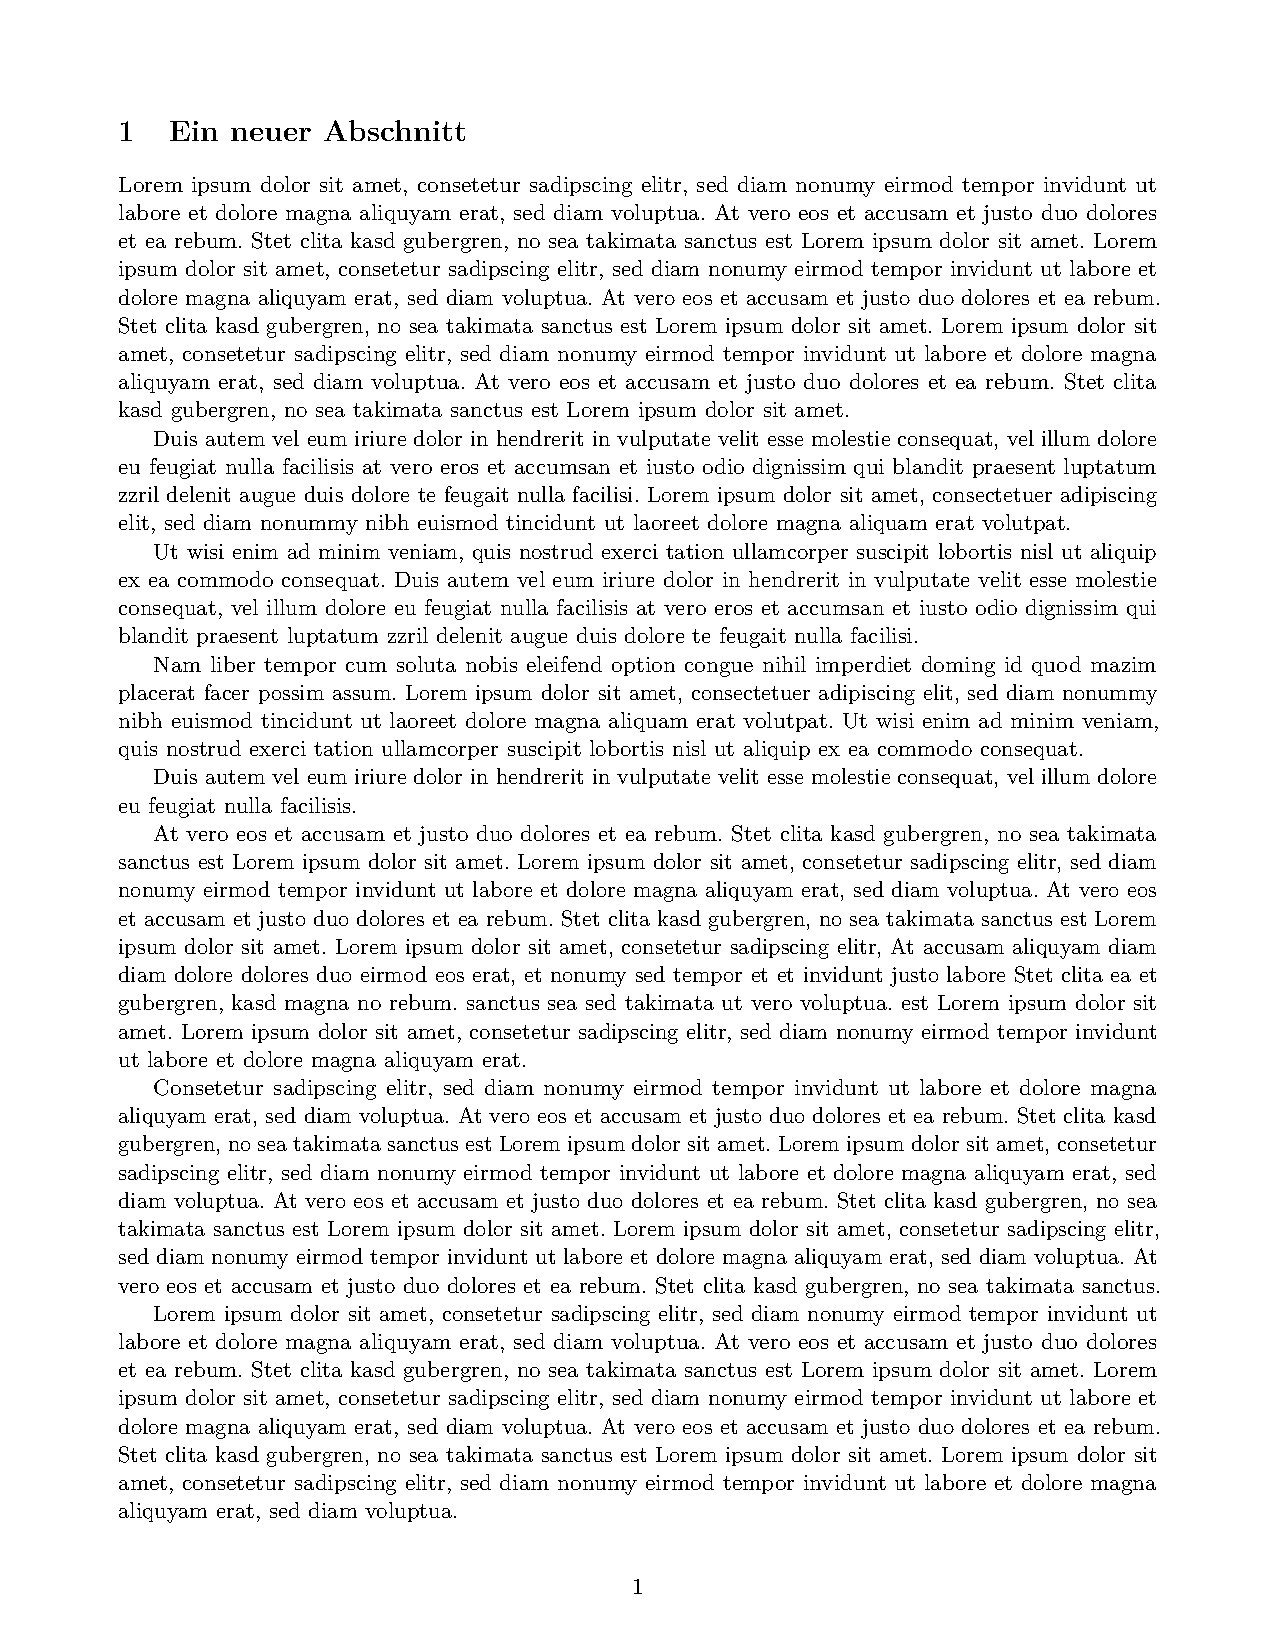
\includegraphics[scale=.23]{Beispiele/Zeilenabstand/Zeilenabstand_normal.pdf}}
\vspace{-5pt}
\caption{einfacher Zeilenabstand}
\end{figure}
\end{minipage}
\pause
\begin{minipage}{.49\textwidth}
\begin{figure}[htp]
\centering
\fbox{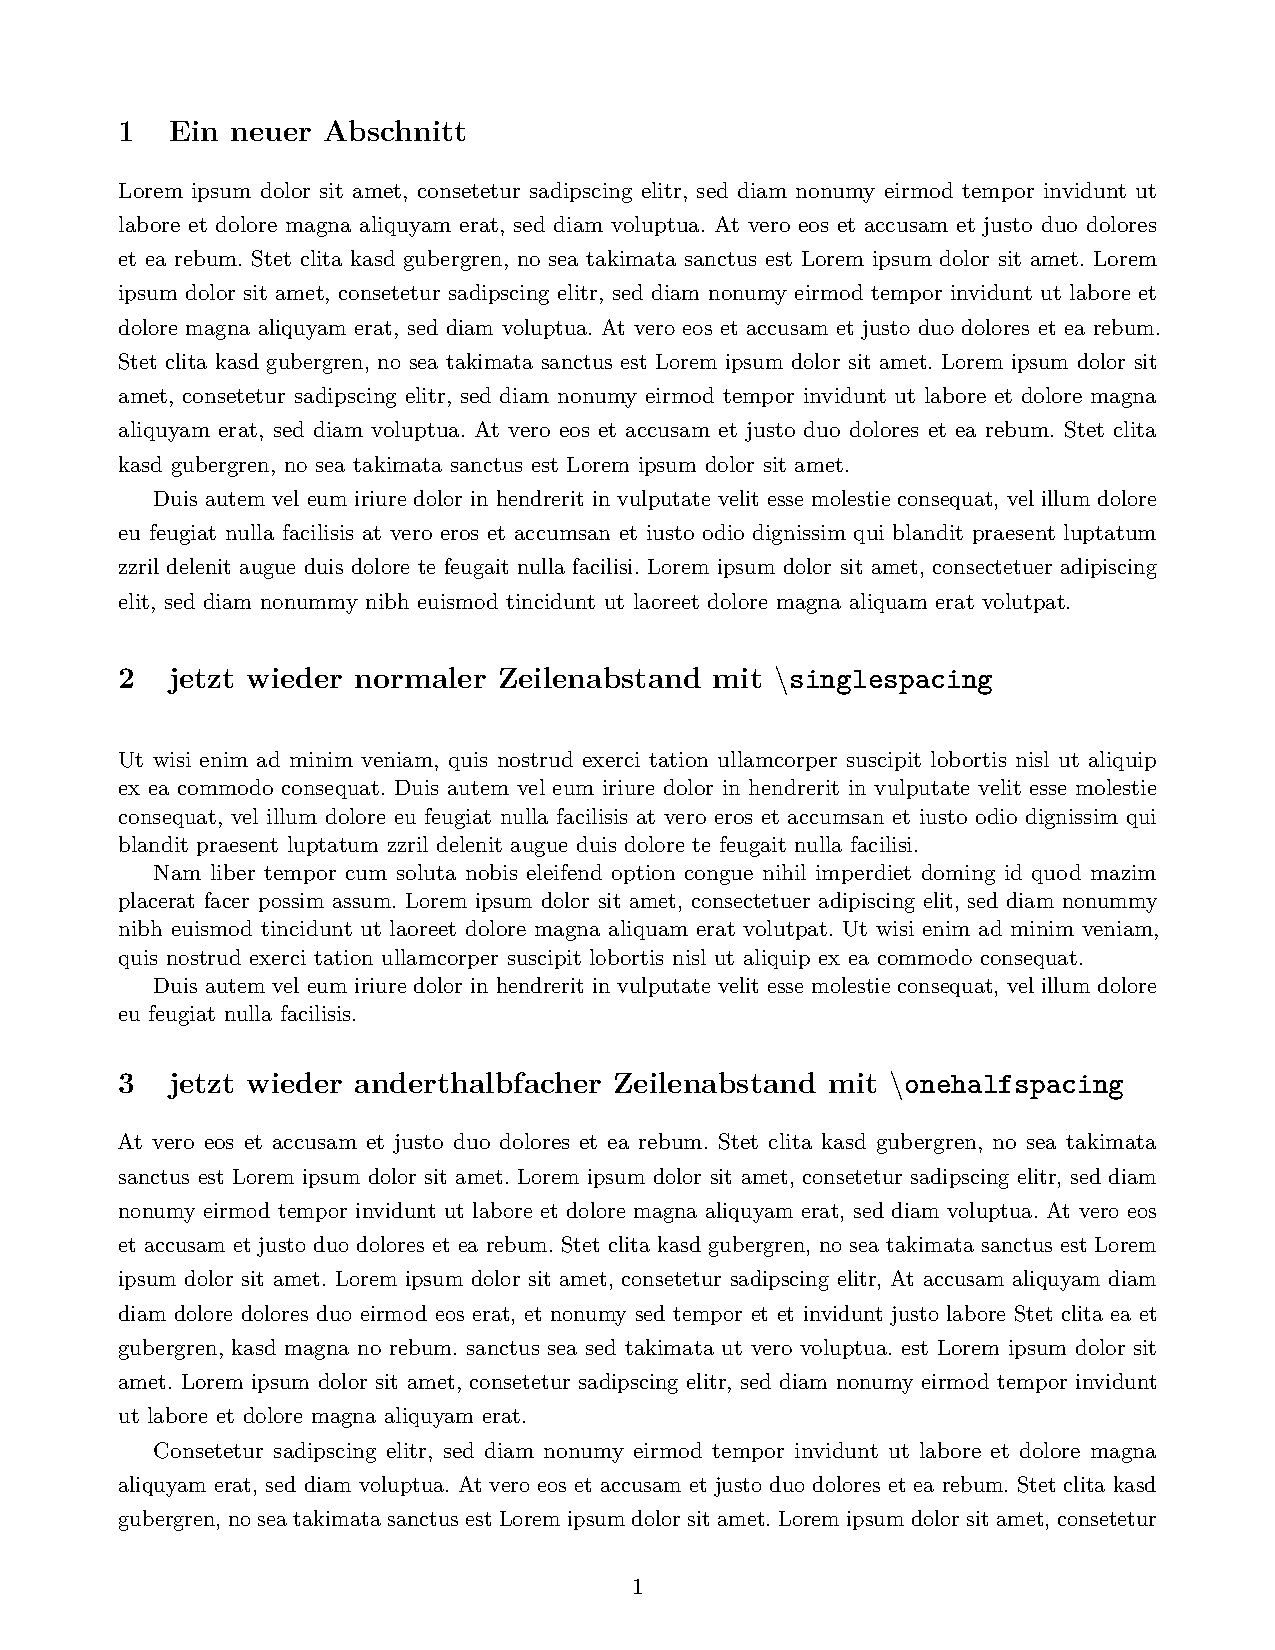
\includegraphics[scale=.23]{Beispiele/Zeilenabstand/Zeilenabstand.pdf}}
\vspace{-5pt}
\caption{einfacher und anderthalbfacher Zeilenabstand}
\end{figure}
\end{minipage}
\end{minipage}
\end{frame}




\subsection{Sonderzeichen}

\begin{frame}[fragile]
\frametitle{Lokalisierung}
Bei der Erstellung deutscher Texte sind folgende Pakete hilfreich:
\begin{description}[<+->]
  \item[babel] zum Einstellen der Sprache. Benötigt für Deutsch den Parameter [ngerman]
    \begin{itemize}
      \item deutsche Anführungszeichen
      \item Automatische Texte werden deutsch (z.B. ``Inhaltsverzeichnis'')
      \item Generiert den Befehl ``\verb+"+'', der deutsche Sonderzeichen erzeugen kann
      \item erlaubt die Verwendung von \verb+\glqq+ und \verb+\grqq+ um Anführungszeichen zu erzeugen
    \end{itemize}
  \item[inputenc] Definiert die Kodierung der .tex-Datei, welche als optionaler Parameter angegeben wird:
    \begin{itemize}
      \item \emph{utf8}: Universeller Standard
     % \item \emph{latin1, applemac}: Frühere Windows / Linux Standards
    \end{itemize}
\end{description}  
\end{frame}



\begin{frame}[fragile]
\frametitle{Anführungszeichen}
Nach dem Einbinden des \texttt{babel}-Paketes stehen folgende Anführungszeichen zur Verfügung: \pause

\begin{itemize}[<+->]
\item Pfeile: \verb+">Hallo"<+ ">Hallo"<
\item Englisch: \verb+``Hallo''+ ``Hallo''
\item Deutsch: \verb+"`Hallo"'+ "`Hallo"' 
\item oder \verb+\glqq+ Hallo \verb+\grqq+ \glqq Hallo\grqq 
\end{itemize}
\end{frame}



\begin{frame}
\frametitle{Lokalisierung}
\begin{description}[<+->]
  \item[fontenc] Sorgt dafür, dass alle 256 Zeichen des europäischen Zeichensatzes dargestellt werden können. Benötigt für europäischen Zeichensatz den optionalen Parameter [T1].
  \item[lmodern] Sorgt für eine Darstellung von Umlauten als Umlaute im PDF-Text und nicht als ``Buchstabe mit Pünktchen darüber''.
\end{description}
\pause
%Pakete für weitere Sonderzeichen können der ``Comprehensive Symbol List'' entnommen werden:
%  \url{http://www.ctan.org/tex-archive/info/symbols/comprehensive/symbols-a4.pdf}\\
%  Dadurch lassen sich tolle Symbole wie diese erstellen: \copyright, \$, \maltese, \checkmark, \PHplumedHead, \BlackBishopOnWhite, \EUR
\end{frame}



\begin{frame}[fragile]
\frametitle{Beispiel eines deutschen Textes}
\begin{lstlisting}[style=Latex]
\documentclass{article}
\usepackage[ngerman]{babel}
\usepackage[utf8]{inputenc}
\usepackage[T1]{fontenc}
\usepackage{lmodern}
\begin{document}
"`Hol mit bitte die Rührschüssel"' sagte Peter.\\
``Sorry I dont speak German'' antwortete Samantha.
\end{document}
\end{lstlisting} \vspace{-20pt}
\pause
Ergibt:
\result{
"`Hol mit bitte die Rührschüssel"' sagte Peter.\\
``Sorry I dont speak German'' antwortete Samantha.
">Standardtext"<
}
\end{frame}

\begin{frame}[fragile]
\frametitle{Beispiel eines deutschen Textes}
\begin{lstlisting}[style=Latex]
\documentclass{article}
\usepackage[ngerman]{babel}
\usepackage[utf8]{inputenc}
\usepackage[T1]{fontenc}
\usepackage{lmodern}
\usepackage[left=2cm,right=2cm,top=2cm,bottom=2cm]{geometry}
\begin{document}
ä Ä ö Ö ü Ü\\
\end{document}
\end{lstlisting} \vspace{-20pt}
\pause
Ergibt:
\result{
ä Ä ö Ö ü Ü\\
}
\end{frame}



\subsection{Seitengröße}
\begin{frame}[fragile,t]
\frametitle{Seitengröße}
Die Papiergröße lässt sich sehr komfortabel mit dem Paket {\tt geometry} einstellen:\vfill
\begin{lstlisting}[style=Latex]
\usepackage[left=2cm,right=2cm,top=2cm,bottom=2cm]{geometry}
\end{lstlisting}
\end{frame}


\begin{frame}[fragile,t]
\frametitle{Beispiel}
\vspace{-10pt}
\begin{minipage}{\textwidth}
\begin{minipage}{.49\textwidth}
%\vspace{-70pt}
\begin{figure}[htp]
\centering
\fbox{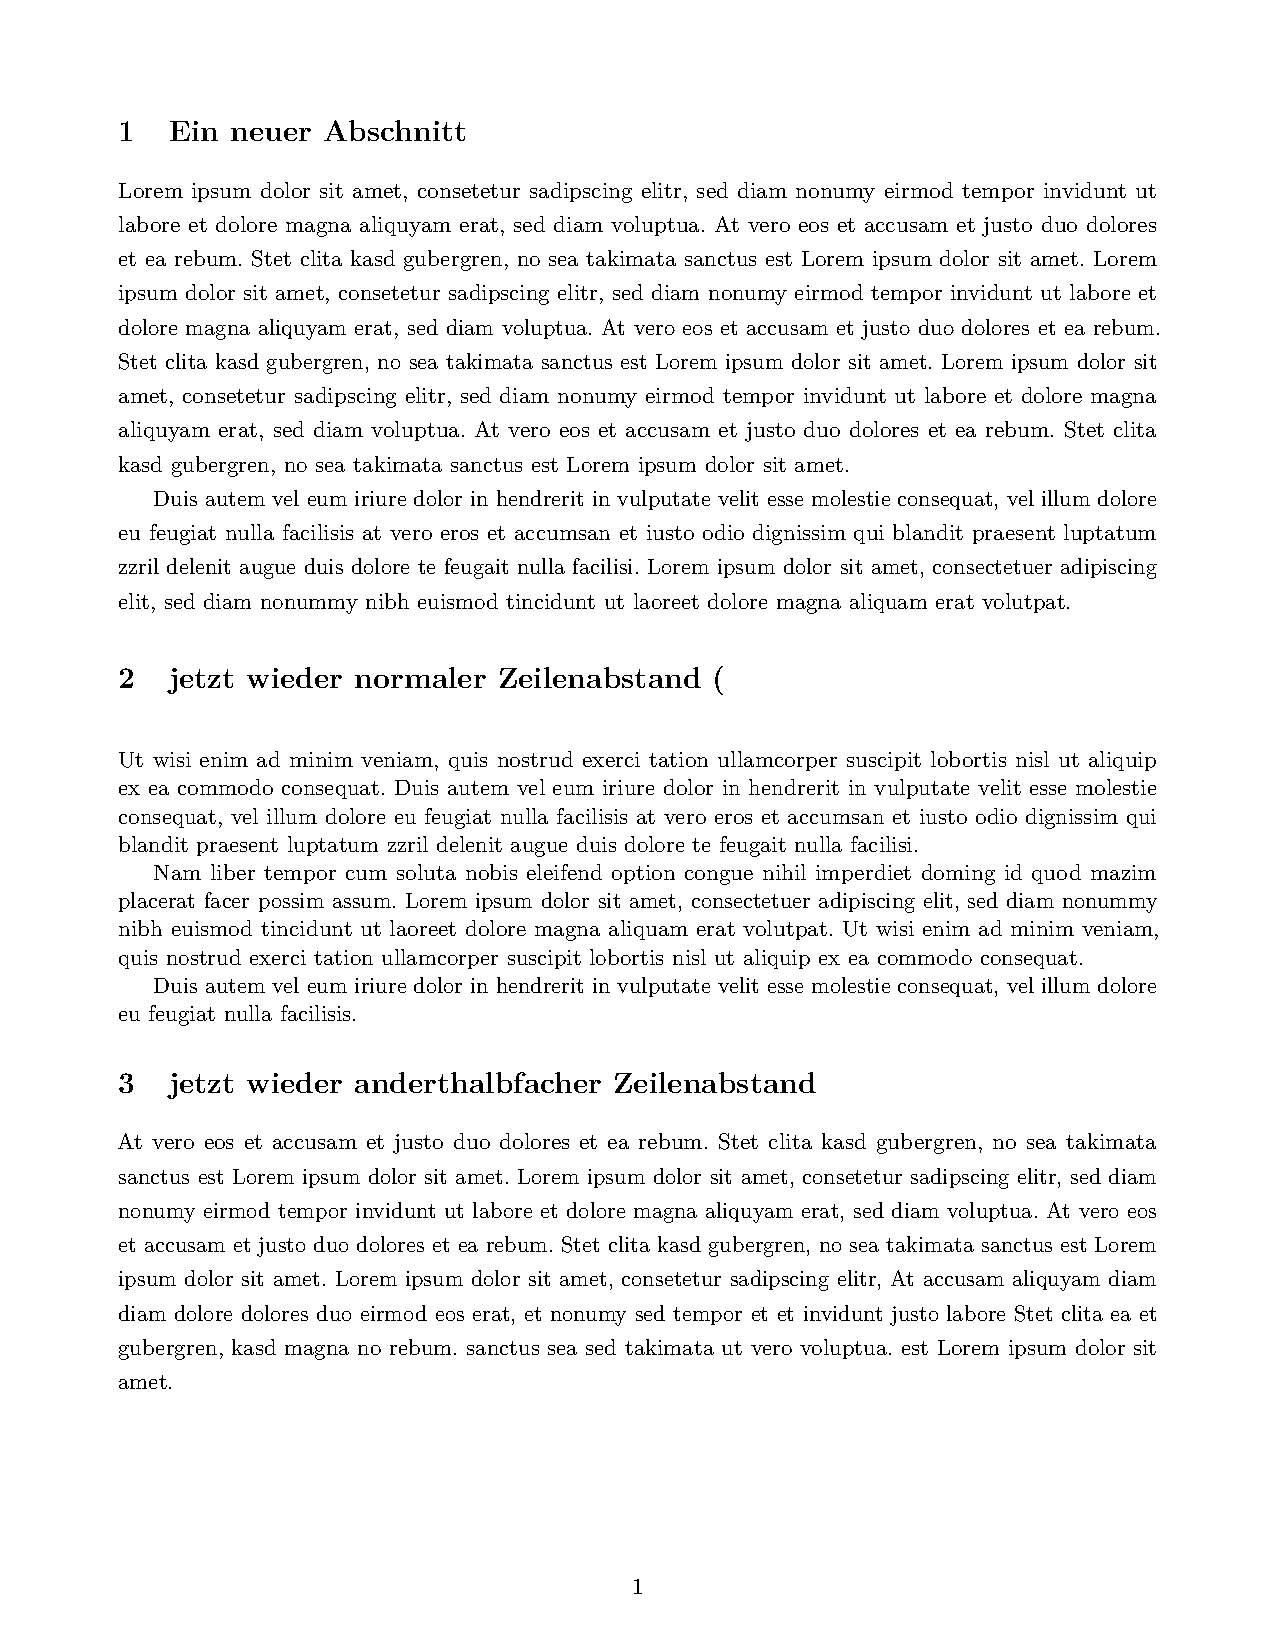
\includegraphics[scale=.23]{Beispiele/Rand/Zeilenabstand.pdf}}
\vspace{-5pt}
\caption{Überall 2cm Abstand zum Rand}
\end{figure}
\end{minipage}
\pause
\begin{minipage}{.49\textwidth}
\begin{figure}[htp]
\centering
\fbox{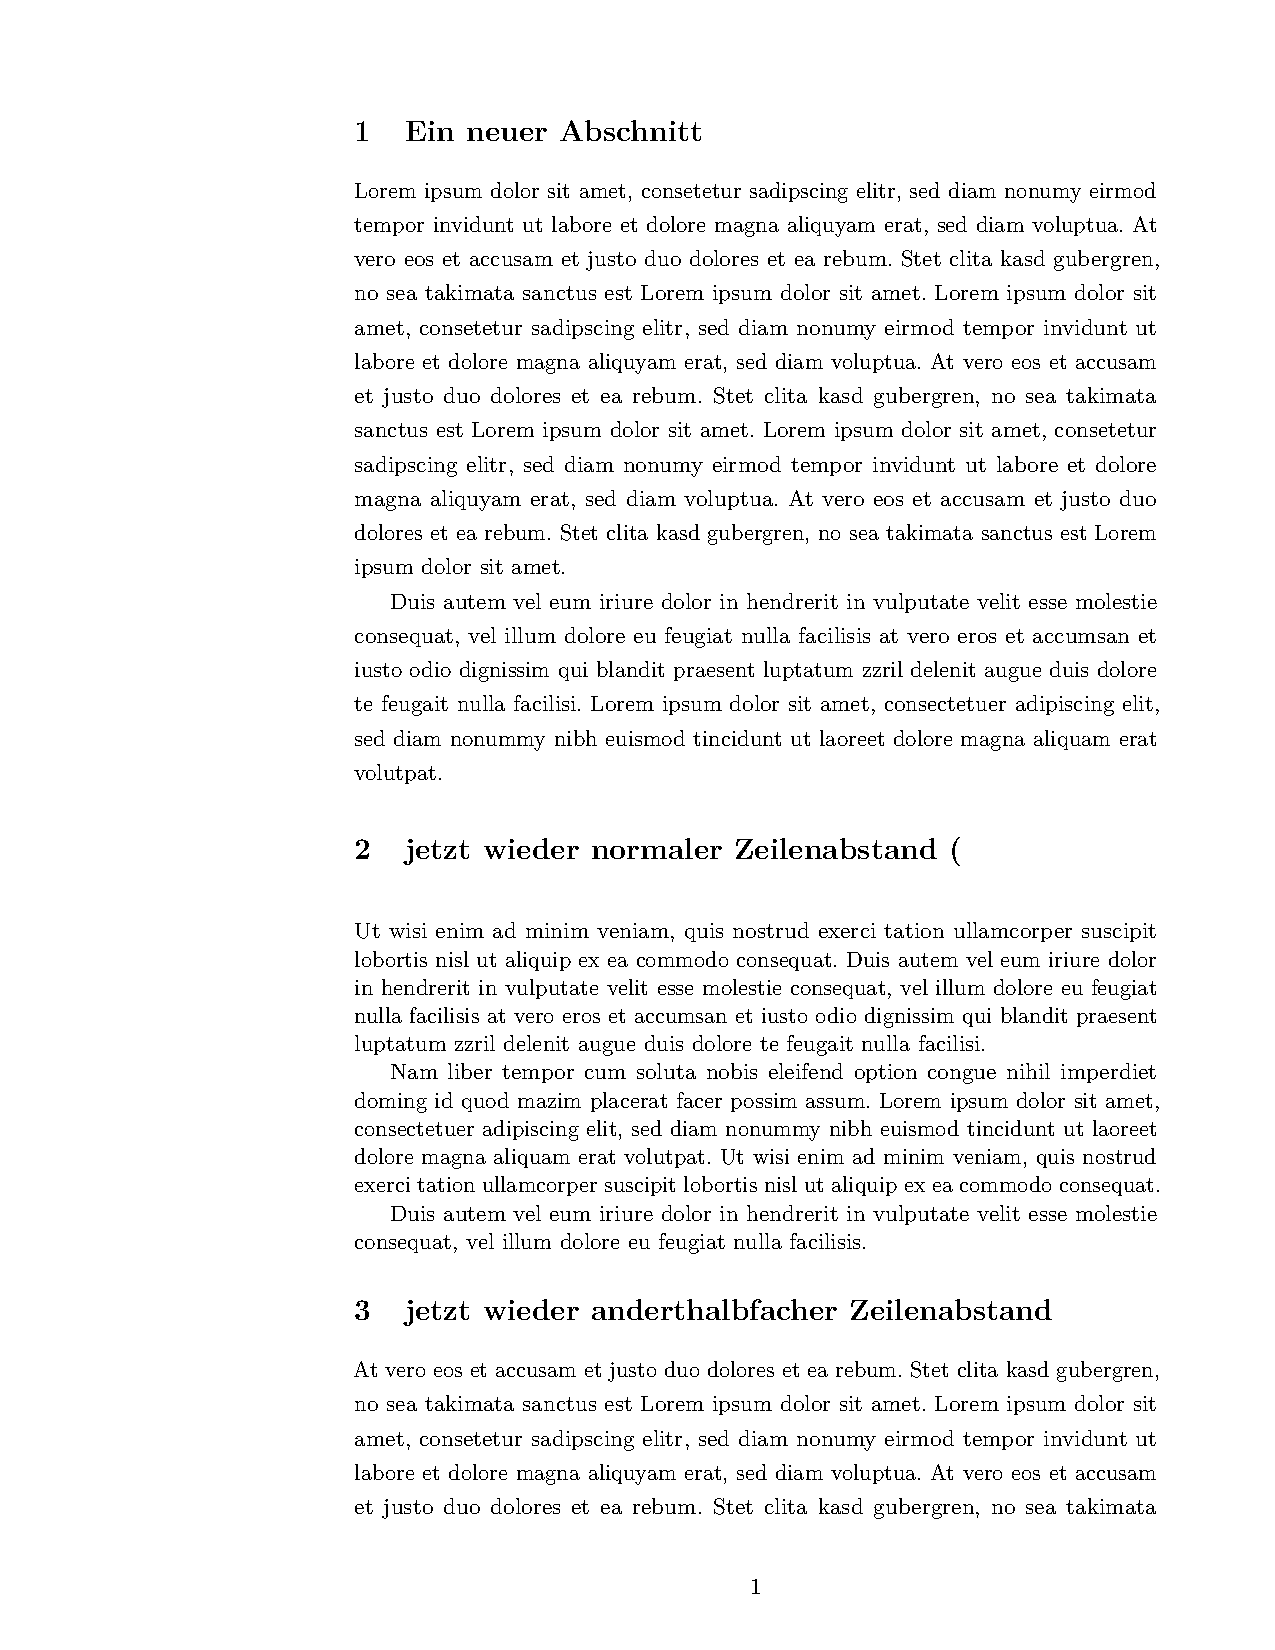
\includegraphics[scale=.23]{Beispiele/Rand/Zeilenabstand_normal.pdf}}
\vspace{-5pt}
\caption{links 6cm Abstand zum Rand}
\end{figure}
\end{minipage}
\end{minipage}
\end{frame}


\subsection{Seitenstile}


\begin{frame}[fragile,t]
\frametitle{Kopf- und Fußzeilen}
\begin{itemize}[<+->]
  \item Das Paket {\tt fancyhdr} ermöglicht eine einfache Verwendung von Kopf- und Fußzeilen
  \item Damit die Seiteneinstellungen korrekt übernommen werden sollten im Quellcode \textbf{zuerst} die Seitengröße durch das geometry-Paket eingestellt werden

  \item Aktivierung durch \begin{center}\lstinline[style=Latex]+\usepackage{fancyhdr}\pagestyle{fancy}+\end{center}
\item Die Syntax für mögliche Positionen lautet:\\
  \begin{center} \small
  \begin{tabular}{|c|} \hline
    \lstinline[style=Latex]+\lhead{<Inhalt>}+  \quad \lstinline[style=Latex]+\chead{<Inhalt>}+  \quad \lstinline[style=Latex]+\rhead{<Inhalt>}+  \\\hline\\
    \huge Text \\\\\hline
    \lstinline[style=Latex]+\lfoot{<Inhalt>}+ \quad \lstinline[style=Latex]+\cfoot{<Inhalt>}+ \quad \lstinline[style=Latex]+\rfoot{<Inhalt>}+ \\\hline
  \end{tabular}
  \end{center}
\end{itemize}
\end{frame}


\begin{frame}[fragile]
\frametitle{Beispiel Kopf und Fußzeile}
\begin{minipage}{.6\textwidth}
{\scriptsize
\begin{lstlisting}[style=Latex]
\documentclass[a4paper]{article}
\usepackage[ngerman]{babel}
\usepackage[utf8]{inputenc}
\usepackage[T1]{fontenc}
\usepackage{lmodern}
\usepackage{fancyhdr}\pagestyle{fancy}
\lhead{Linke Kopfzeile}
\rhead{rechte Kopfzeile}
\lfoot{linke Fußzeile} 
\cfoot{}
\rfoot{Seitenzahl: \thepage}
\begin{document}
"`Hol mit bitte die Rührschüssel"' sagte Peter.\\
``Sorry I dont speak German'' antwortete Samantha.
\end{document}
\end{lstlisting}}

\end{minipage}
\pause
\begin{minipage}{.39\textwidth}

\begin{figure}[htp]
\centering
\fbox{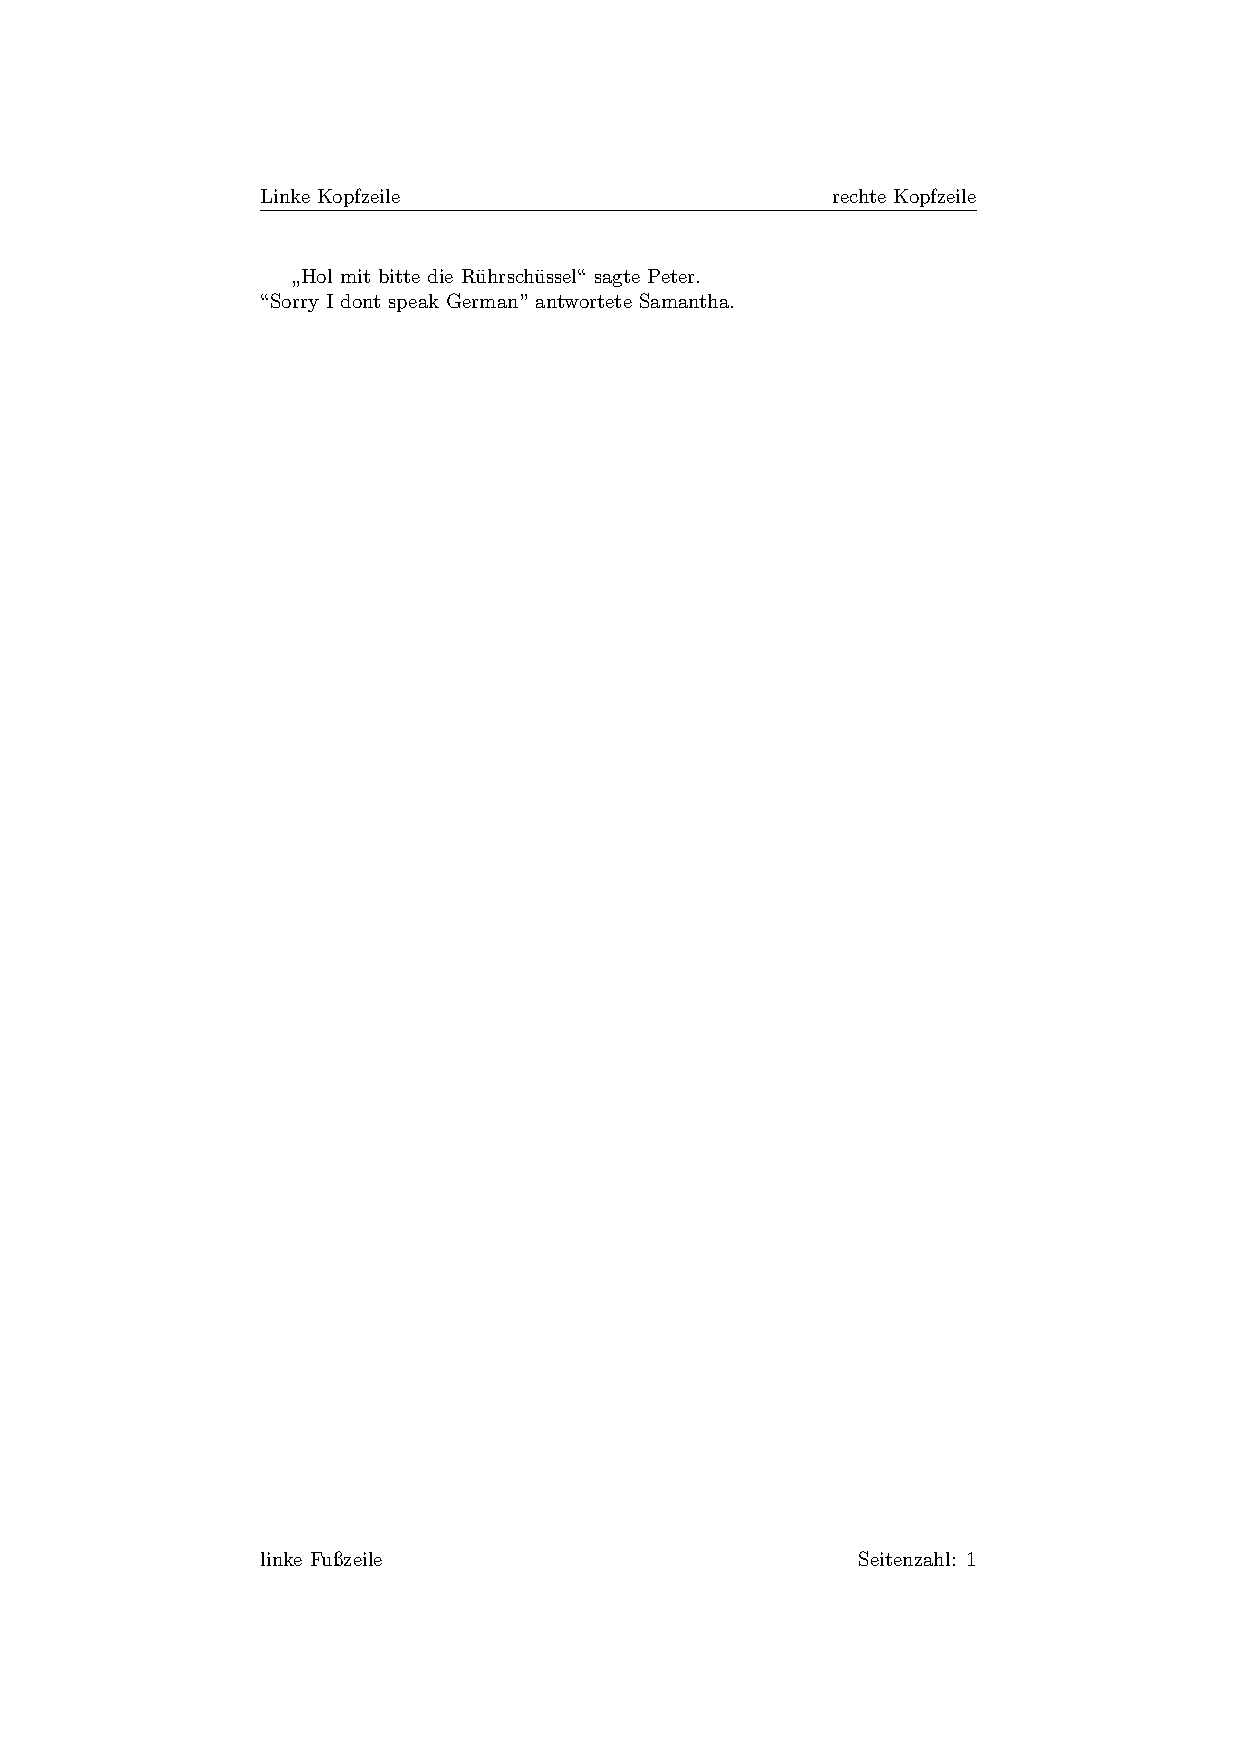
\includegraphics[scale=.25]{Beispiele/KopfundFusszeile/KopfundFusszeile.pdf}}
\vspace{-20pt}
\caption{Kopf- und Fußzeile}
\end{figure}

\end{minipage}
\end{frame}



\begin{frame}[fragile]
\frametitle{Verwendung von Zählern}
Anzeigen von bestimmten Elementen in Kopf- oder Fußzeile:
\begin{itemize}[<+->]
  	\item Kapitel (\lstinline[style=Latex]+\section+)	
	\item Unterkapitel (\lstinline[style=Latex]+\subsection+) , Unterunterkapitel (\lstinline[style=Latex]+\subsubsection+)
	\item Seitenanzahl (\lstinline[style=Latex]+\thepage+)
	\item Datum der Kompilierung (\lstinline[style=Latex]+\today+)
\end{itemize}
\end{frame}

\begin{frame}[fragile]
\frametitle{Seitennummerierung}
\begin{itemize}[<+->]
  \item Die Seitennummerierung wird festgelegt mit \\
  \quad \lstinline[style=Latex]+\pagenumbering{<Stil>}+
  \item Mögliche Stile sind
  \begin{itemize}
    \item \texttt{\textbf{arabic}}: Arabische Zahlen (Standard)
    \item \texttt{\textbf{roman}}/\texttt{\textbf{Roman}}: kleine/große römische Ziffern
    \item \texttt{\textbf{alph}}/\texttt{\textbf{Alph}}: Kleinbuchstaben/Großbuchstaben
  \end{itemize}
  \item Dies kann an jeder Stelle im Text geändert werden. Dabei wird jedoch der Zähler auf 1 gesetzt.
  \item Ändern des Zählers durch \lstinline[style=Latex]+\setcounter{page}{<Seitennummer>}+
\end{itemize}
\end{frame}

\subsection{Schriftbild}



\begin{frame}[fragile,t]
\frametitle{Schriftsatz}
Die Schrift in einer Umgebung <Text> lässt sich wie folgt anpassen:
\begin{itemize}[<+->]
  \item Schriftart
  \begin{itemize}
    \item \lstinline[style=Latex]+\textrm{<Text>}+: {\rmfamily Roman-Schrift}
    \item \lstinline[style=Latex]+\texttt{<Text>}+: {\ttfamily Schreibmaschinenschrift}
   % \item \lstinline[style=Latex]+\sf{<Text>}+: {\sffamily Serifenlose Schrift}
  \end{itemize}  
  \item Form:
  \begin{itemize}
    \item \lstinline[style=Latex]+\textit{<Text>}+: {\itshape Kursivschrift}
   % \item \lstinline[style=Latex]+\slshape+: {\slshape Geneigte Schrift}
   % \item \lstinline[style=Latex]+\scshape+: {\scshape Kapitälchen}
   % \item \lstinline[style=Latex]+\upshape+: {\upshape Aufrechte Schrift }
  \end{itemize}
  \item Serie:
  \begin{itemize}
    \item {\lstinline[style=Latex]+\textbf{<Text>}+: \bfseries Fettschrift}
   % \item \lstinline[style=Latex]+\mdseries+: {\mdseries Standard}
  \end{itemize}
\end{itemize}~\\
\pause
{\scriptsize
\begin{minipage}{.55\textwidth}
\begin{lstlisting}[style=Latex]
\texttt{Schreibmaschinenschrift}\\
\texttt{Schreib\textbf{maschinen}schrift}\\
\texttt{kursive Schrift}
\end{lstlisting}
\end{minipage}}\pause~
\begin{minipage}{.39\textwidth}
\result{
\texttt{Schreibmaschinenschrift}\\
\texttt{Schreib\textbf{maschinen}schrift}\\
\texttt{kursive Schrift}
}
\end{minipage}

\end{frame}


\begin{comment}
\begin{frame}[fragile]
\frametitle{Schriftsatz}
\begin{itemize}[<+->]
  \item Möchte man nicht die gesamte Umgebung ändern, sondern nur ein Wort o.ä., so bietet sich
\begin{lstlisting}[style=Latex] 
\text<Kuerzel>{<Text>} 
\end{lstlisting}\vspace{-20pt}
an. Als Kürzel gelten die ersten beiden Buchstaben der oben genannten Befehle (rm, it, up, ...).
\end{itemize}
\pause
\begin{lstlisting}[style=Latex]
{\ttfamily In einer Umgebung} \\
\texttt{So gehts auch} \\
\texttt{\sffamily Was passiert wohl hier?}
\end{lstlisting}\vspace{-20pt}
\pause
\result{
{\ttfamily In einer Umgebung} \\
\texttt{So gehts auch} \\
\texttt{\sffamily Was passiert wohl hier?}}
\end{frame}
\end{comment}

\begin{frame}[fragile]
\frametitle{Schriftsatz}
\begin{itemize}[<+->]
  \item Schriftgröße:
  \begin{center}\begin{tabular}{ll}
    				\lstinline[style=Latex]+\tiny+: 			& \tiny winzig\\
    \onslide<2->	\lstinline[style=Latex]+\scriptsize+:		& \onslide<2-> \scriptsize sehr klein\\
    \onslide<3->	\lstinline[style=Latex]+\footnotesize+:	& \onslide<3-> \footnotesize Fußnote\\
    \onslide<4-> \lstinline[style=Latex]+\small+:			& \onslide<4-> \small klein\\
    \onslide<5-> \lstinline[style=Latex]+\normalsize+:		& \onslide<5-> \normalsize normal\\
    \onslide<6-> \lstinline[style=Latex]+\large+:			& \onslide<6-> \large groß\\
    \onslide<7-> \lstinline[style=Latex]+\Large+:			& \onslide<7-> \Large Größer\\
    \onslide<8-> \lstinline[style=Latex]+\LARGE+:			& \onslide<8-> \LARGE sehr groß\\
    \onslide<9-> \lstinline[style=Latex]+\huge+:			& \onslide<9-> \huge riesig\\
    \onslide<10-> \lstinline[style=Latex]+\Huge+:			& \onslide<10-> \Huge gigantisch
  \end{tabular}\end{center}
 % \item<11-> Eigene Schriftgröße: \lstinline[style=Latex]+\fontsize{<size>}{<skip>}\selectfont+\\
  %  Dabei ist \lstinline[style=Latex]+<size>+ die Schriftgröße und \lstinline[style=Latex]+<skip>+ der Zeilenabstand in pt.
\end{itemize}
\end{frame}



\begin{frame}[fragile]
  \frametitle{Beispiel}
  \begin{lstlisting}[style=Latex]
\textbf{\large{ Es ist schwer, Internetzitate auf Echtheit zu testen}} \\
\scriptsize{\texttt{Abraham Lincoln}}
\end{lstlisting}
      \textbf{\large{ Es ist schwer, Internetzitate auf Echtheit zu testen}} \\
      \scriptsize{\texttt{Abraham Lincoln}}
\end{frame}

\begin{comment}
\begin{frame}[fragile]
  \frametitle{Farben}
  \begin{itemize}[<+->]
  \item Das \texttt{color}-Paket erlaubt die Benutzung von Farben in \LaTeX
  \item Definiert werden Farben mittels 
    \begin{center} \lstinline[style=Latex]+\definecolor{<Name>}{<System>}{<Spezifikation>}+ \end{center} \pause
    Systeme:
    \begin{itemize}
    \item \texttt{rgb} für RGB-Farben
    \item \texttt{gray} für Grautöne
    \item weitere Spezialsysteme, z.B. \texttt{html, cmyk}
    \end{itemize}
  \item Vordefiniert sind die Farben \textbf{black, white, red, green, blue, cyan, magenta, yellow}
  \item Außerdem sind nun verfügbar:
    \begin{itemize}
    \item \lstinline[style=Latex]+\textcolor{<Farbe>}{<Text>}+ färbt den eingefügten Text
    \item \lstinline[style=Latex]+\color{<Farbe>}+ färbt allen Text in der aktuellen Umgebung
    \item \lstinline[style=Latex]+\pagecolor{<Farbe>}+ färbt den Hintergrund der aktuellen Seite
    \item \lstinline[style=Latex]+\colorbox{<Farbe>}{<Text>}+ färbt den Hintergrund des Textes
    \item \lstinline[style=Latex]+\fcolorbox{<Farbe1>}{<Farbe2>}{<Text>}+ umrandet den Text mit Farbe1 und hinterlegt ihn mit Farbe2      
    \end{itemize}
  \end{itemize}
\end{frame}

\begin{frame}[fragile,t]
  \frametitle{Beispiel}
  \begin{lstlisting}[style=Latex]
    \definecolor{darkblue}{rgb}{0,0,.5}
    \definecolor{mygray}{gray}{.75}
    \textcolor{darkblue}{Hallo }
    \colorbox{mygray}{Welt}
  \end{lstlisting}
  \pause
  \vspace{-20pt}
\result{
  \definecolor{darkblue}{rgb}{0,0,.5}
  \definecolor{mygray}{gray}{.75}
  \textcolor{darkblue}{Hallo }
  \colorbox{mygray}{Welt}}
\end{frame}
\end{comment}



\subsection{Whitespaces}

\begin{frame}[fragile]
\frametitle{Zeilenumbrüche}
\begin{itemize}[<+->]
  \item ein Zeilenumbruch wird mittels \lstinline[style=Latex]+\\+ bzw. \lstinline[style=Latex]+\newline+ erzeugt.
  \item \lstinline[style=Latex]+\\+ kann als optionalen Parameter einen Abstand zur nächsten Zeile haben:\\
    \lstinline[style=Latex]+\\[5cm]+
 % \item \lstinline[style=Latex]+\linebreak[<Dringlichkeit>]+ erzeugt einen Zeilenumbruch, bei dem die aktuelle Zeile noch aufgefüllt wird.\\
 % Diese Dringlichkeit ist ein Wert zwischen 0 und 4.
  \item Zeilenumbrüche funktionieren nur nach Text, nach einer Umgebung muss unter Umständen ein Abstand (Tilde) eingefügt werden.
\end{itemize}
\end{frame}

\begin{frame}[fragile]
\frametitle{Absätze}
\begin{itemize}[<+->]
  \item Ein neuer Absatz wird durch eine Leerzeile erzeugt:
  \item neue Absätze werden standardmäßig eingerückt. Dieser Abstand wird mit \lstinline[style=Latex]+\parindent+ definiert.
  \item \lstinline[style=Latex]+\indent+ bzw. \lstinline[style=Latex]+\noindent+ fügen manuell diesen Abstand ein oder verhindern ihn für den aktuellen Absatz.
  \item Um die Einrückung im Dokument zu deaktivieren reicht es nach \lstinline[style=Latex]+\begin{document}+
\begin{center}
    \lstinline[style=Latex]+\setlength{\parindent}{0cm}+ 
\end{center}
zu schreiben
\end{itemize}
\end{frame}

\begin{comment}
\begin{frame}[fragile]
\frametitle{horizontaler Abstand}
\begin{itemize}[<+->]
  \item \lstinline[style=Latex]+\hspace{<Abstand>}+ erzeugt einen horizontalen Abstand.
  \item Beispiele: \\
    \lstinline[style=Latex]+Hallo \hspace{3ex} Welt+: Hallo \hspace{3ex} Welt\\
    \lstinline[style=Latex]+Hallo \hspace{-3ex} Welt+: Hallo \hspace{-3ex} Welt\\
  \item definierte Abstände sind (jeweils in Geviert)\\[1ex]
    \hspace{-3ex}\begin{tabular}{l||c|c|c|c|c|c}
    Befehl & \lstinline[style=Latex]+\!+ & \lstinline[style=Latex]+\,+ & \lstinline[style=Latex]+\;+ & \lstinline[style=Latex]+\ + & \lstinline[style=Latex]+\quad+ & \lstinline[style=Latex]+\qquad+ \\\hline
    Abstand & -3/18 & 3/18 & 5/18 & 1/3 & 1 & 2
    \end{tabular}
  \item \lstinline[style=Latex]+\hfill+ füllt so, dass der restliche Text rechtsbündig abschließt. Mehrere Aufrufe in einer Zeile ``teilen'' sich den Rest. Ebenso \lstinline[style=Latex]+\dotfill+ und \lstinline[style=Latex]+\hrulefill+.
\noindent
\begin{lstlisting}[frame=single]
T1 \hfill T2 \dotfill T3 \hrulefill T4
\end{lstlisting} 
\pause
\vspace{-20pt}
\result{ 
    T1 \hfill T2 \dotfill T3 \hrulefill T4}
\end{itemize}
\end{frame}
\end{comment}

\begin{frame}[fragile]
\frametitle{vertikaler Abstand}
\begin{itemize}[<+->]
  \item Füllen des Rests der Seite mit Leerzeilen
  \begin{itemize}
     % \item \lstinline[style=Latex]+\pagebreak+: wie \lstinline[style=Latex]+\linebreak+
     % \item \lstinline[style=Latex]+\vspace+: wie \lstinline[style=Latex]+\hspace+
      \item \lstinline[style=Latex]+\vfill+%wie \lstinline[style=Latex]+\hfill+
    \end{itemize}\vfill
  \item Erstellen einer neuen Seite:
    \begin{itemize}
      \item \lstinline[style=Latex]+\newpage+%: Erzeugt eine neue Seite% wie \lstinline[style=Latex]+\newline+
     % \item \lstinline[style=Latex]+\pagebreak+: wie \lstinline[style=Latex]+\linebreak+
     % \item \lstinline[style=Latex]+\vspace+: wie \lstinline[style=Latex]+\hspace+
     % \item \lstinline[style=Latex]+\vfill+: wie \lstinline[style=Latex]+\hfill+
    \end{itemize}\vfill
  \item definierte Abstände nach Absätzen: \\
    \lstinline[style=Latex]+\bigskip+\hfill \lstinline[style=Latex]+\medskip+\hfill \lstinline[style=Latex]+\smallskip+ \hfill\,
\vfill
  \item Abstand nach einem Zeilenumbruch durch:\\
    \lstinline[style=Latex]+\\[2cm]+
\end{itemize}
\end{frame}

\subsection{Positionierung}

\begin{frame}[fragile]
\frametitle{Positionierung}
\begin{itemize}[<+->]
\item die \texttt{center}-Umgebung ist direkt von sich aus zentriert
\item analog dazu existiert die \texttt{flushright}- bzw. \texttt{flushleft}-Umgebung
\end{itemize}
\end{frame}

\begin{frame}[fragile,t]
  \frametitle{Beispiel}
  \begin{lstlisting}[style=Latex]
\begin{center}
Dieser Text ist zentriert,
\end{center}
\begin{flushright}
dieser hier nach rechts ausgerichtet.
\end{flushright}
\end{lstlisting}\vspace{-20pt}
  \pause
\result{
  \begin{center}
    Dieser Text ist zentriert,
  \end{center}
  \begin{flushright}
    dieser hier nach rechts ausgerichtet.
  \end{flushright}}
\end{frame}

\subsection{Gliederung}


\begin{frame}[fragile]
\frametitle{Gliederungsebenen}
\begin{itemize}[<+->]
  \item Syntax: \lstinline[style=Latex]+\<Ebene>[<Kurzform>]{<Titel>}+
  \item Mögliche Ebenen sind:
  \begin{itemize}
    \item part: Teil (nur bei book)
    \item chapter: Kapitel (nur bei book und report)
    \item section: Abschnitt
    \item subsection: Unterabschnitt
    \item subsubsection: Unterunterabschnitt
    \item paragraph: Absatz
    \item subparagraph: Unterabsatz
  \end{itemize}
  \item Der optionale Parameter <Kurzform> taucht als Name im Inhaltsverzeichnis und im Header auf.
  \item Die Nummerierung kann mit ``*'' unterdrückt werden: \lstinline[style=Latex]+\section*{Nummerlos}+
\end{itemize}
\end{frame}
